% $Id: conference_paper.tex,v 1.8 2006/09/06 19:09:21 borning Exp $

%% bare_conf.tex 
%% V1.2
%% 2002/11/18
%% by Michael Shell
%% mshell@ece.gatech.edu
%% 
%% NOTE: This text file uses MS Windows line feed conventions. When (human)
%% reading this file on other platforms, you may have to use a text
%% editor that can handle lines terminated by the MS Windows line feed
%% characters (0x0D 0x0A).
%% 
%% This is a skeleton file demonstrating the use of IEEEtran.cls 
%% (requires IEEEtran.cls version 1.6b or later) with an IEEE conference paper.
%% 
%% Support sites:
%% http://www.ieee.org
%% and/or
%% http://www.ctan.org/tex-archive/macros/latex/contrib/supported/IEEEtran/ 
%%
%% This code is offered as-is - no warranty - user assumes all risk.
%% Free to use, distribute and modify.

% *** Authors should verify (and, if needed, correct) their LaTeX system  ***
% *** with the testflow diagnostic prior to trusting their LaTeX platform ***
% *** with production work. IEEE's font choices can trigger bugs that do  ***
% *** not appear when using other class files.                            ***
% Testflow can be obtained at:
% http://www.ctan.org/tex-archive/macros/latex/contrib/supported/IEEEtran/testflow


% Note that the a4paper option is mainly intended so that authors in
% countries using A4 can easily print to A4 and see how their papers will
% look in print. Authors are encouraged to use U.S. letter paper when 
% submitting to IEEE. Use the testflow package mentioned above to verify
% correct handling of both paper sizes by the author's LaTeX system.
%
% Also note that the "draftcls" or "draftclsnofoot", not "draft", option
% should be used if it is desired that the figures are to be displayed in
% draft mode.
%
% This paper can be formatted using the peerreviewca
% (instead of conference) mode.
%\documentclass[conference]{IEEEtran}
% If the IEEEtran.cls has not been installed into the LaTeX system files, 
% manually specify the path to it:
\documentclass[conference]{./IEEEtran} 


% some very useful LaTeX packages include:

\usepackage{cite}      % Written by Donald Arseneau
                        % V1.6 and later of IEEEtran pre-defines the format
                        % of the cite.sty package \cite{} output to follow
                        % that of IEEE. Loading the cite package will
                        % result in citation numbers being automatically
                        % sorted and properly "ranged". i.e.,
                        % [1], [9], [2], [7], [5], [6]
                        % (without using cite.sty)
                        % will become:
                        % [1], [2], [5]--[7], [9] (using cite.sty)
                        % cite.sty's \cite will automatically add leading
                        % space, if needed. Use cite.sty's noadjust option
                        % (cite.sty V3.8 and later) if you want to turn this
                        % off. cite.sty is already installed on most LaTeX
                        % systems. The latest version can be obtained at:
                        % http://www.ctan.org/tex-archive/macros/latex/contrib/supported/cite/

\usepackage{graphicx}  % Written by David Carlisle and Sebastian Rahtz
                        % Required if you want graphics, photos, etc.
                        % graphicx.sty is already installed on most LaTeX
                        % systems. The latest version and documentation can
                        % be obtained at:
                        % http://www.ctan.org/tex-archive/macros/latex/required/graphics/
                        % Another good source of documentation is "Using
                        % Imported Graphics in LaTeX2e" by Keith Reckdahl
                        % which can be found as esplatex.ps and epslatex.pdf
                        % at: http://www.ctan.org/tex-archive/info/
% NOTE: for dual use with latex and pdflatex, instead load graphicx like:
%\ifx\pdfoutput\undefined
%\usepackage{graphicx}
%\else
%\usepackage[pdftex]{graphicx}
%\fi
% However, be warned that pdflatex will require graphics to be in PDF
% (not EPS) format and will preclude the use of PostScript based LaTeX
% packages such as psfrag.sty and pstricks.sty. IEEE conferences typically
% allow PDF graphics (and hence pdfLaTeX). However, IEEE journals do not
% (yet) allow image formats other than EPS or TIFF. Therefore, authors of
% journal papers should use traditional LaTeX with EPS graphics.
%
% The path(s) to the graphics files can also be declared: e.g.,
\graphicspath{{./figs/}}

% if the graphics files are not located in the same directory as the
% .tex file. This can be done in each branch of the conditional above
% (after graphicx is loaded) to handle the EPS and PDF cases separately.
% In this way, full path information will not have to be specified in
% each \includegraphics command.
%
% Note that, when switching from latex to pdflatex and vice-versa, the new
% compiler will have to be run twice to clear some warnings.


%\usepackage{psfrag}    % Written by Craig Barratt, Michael C. Grant,
                        % and David Carlisle
                        % This package allows you to substitute LaTeX
                        % commands for text in imported EPS graphic files.
                        % In this way, LaTeX symbols can be placed into
                        % graphics that have been generated by other
                        % applications. You must use latex->dvips->ps2pdf
                        % workflow (not direct pdf output from pdflatex) if
                        % you wish to use this capability because it works
                        % via some PostScript tricks. Alternatively, the
                        % graphics could be processed as separate files via
                        % psfrag and dvips, then converted to PDF for
                        % inclusion in the main file which uses pdflatex.
                        % Docs are in "The PSfrag System" by Michael C. Grant
                        % and David Carlisle. There is also some information 
                        % about using psfrag in "Using Imported Graphics in
                        % LaTeX2e" by Keith Reckdahl which documents the
                        % graphicx package (see above). The psfrag package
                        % and documentation can be obtained at:
                        % http://www.ctan.org/tex-archive/macros/latex/contrib/supported/psfrag/

%\usepackage{subfigure} % Written by Steven Douglas Cochran
                        % This package makes it easy to put subfigures
                        % in your figures. i.e., "figure 1a and 1b"
                        % Docs are in "Using Imported Graphics in LaTeX2e"
                        % by Keith Reckdahl which also documents the graphicx
                        % package (see above). subfigure.sty is already
                        % installed on most LaTeX systems. The latest version
                        % and documentation can be obtained at:
                        % http://www.ctan.org/tex-archive/macros/latex/contrib/supported/subfigure/

\usepackage{url}       % Written by Donald Arseneau
                        % Provides better support for handling and breaking
                        % URLs. url.sty is already installed on most LaTeX
                        % systems. The latest version can be obtained at:
                        % http://www.ctan.org/tex-archive/macros/latex/contrib/other/misc/
                        % Read the url.sty source comments for usage information.

%\usepackage{stfloats}  % Written by Sigitas Tolusis
                        % Gives LaTeX2e the ability to do double column
                        % floats at the bottom of the page as well as the top.
                        % (e.g., "\begin{figure*}[!b]" is not normally
                        % possible in LaTeX2e). This is an invasive package
                        % which rewrites many portions of the LaTeX2e output
                        % routines. It may not work with other packages that
                        % modify the LaTeX2e output routine and/or with other
                        % versions of LaTeX. The latest version and
                        % documentation can be obtained at:
                        % http://www.ctan.org/tex-archive/macros/latex/contrib/supported/sttools/
                        % Documentation is contained in the stfloats.sty
                        % comments as well as in the presfull.pdf file.
                        % Do not use the stfloats baselinefloat ability as
                        % IEEE does not allow \baselineskip to stretch.
                        % Authors submitting work to the IEEE should note
                        % that IEEE rarely uses double column equations and
                        % that authors should try to avoid such use.
                        % Do not be tempted to use the cuted.sty or
                        % midfloat.sty package (by the same author) as IEEE
                        % does not format its papers in such ways.

%\usepackage{amsmath}   % From the American Mathematical Society
                        % A popular package that provides many helpful commands
                        % for dealing with mathematics. Note that the AMSmath
                        % package sets \interdisplaylinepenalty to 10000 thus
                        % preventing page breaks from occurring within multiline
                        % equations. Use:
%\interdisplaylinepenalty=2500
                        % after loading amsmath to restore such page breaks
                        % as IEEEtran.cls normally does. amsmath.sty is already
                        % installed on most LaTeX systems. The latest version
                        % and documentation can be obtained at:
                        % http://www.ctan.org/tex-archive/macros/latex/required/amslatex/math/



% Other popular packages for formatting tables and equations include:

%\usepackage{array}
% Frank Mittelbach's and David Carlisle's array.sty which improves the
% LaTeX2e array and tabular environments to provide better appearances and
% additional user controls. array.sty is already installed on most systems.
% The latest version and documentation can be obtained at:
% http://www.ctan.org/tex-archive/macros/latex/required/tools/

% Mark Wooding's extremely powerful MDW tools, especially mdwmath.sty and
% mdwtab.sty which are used to format equations and tables, respectively.
% The MDWtools set is already installed on most LaTeX systems. The lastest
% version and documentation is available at:
% http://www.ctan.org/tex-archive/macros/latex/contrib/supported/mdwtools/


% V1.6 of IEEEtran contains the IEEEeqnarray family of commands that can
% be used to generate multiline equations as well as matrices, tables, etc.


% Also of notable interest:

% Scott Pakin's eqparbox package for creating (automatically sized) equal
% width boxes. Available:
% http://www.ctan.org/tex-archive/macros/latex/contrib/supported/eqparbox/



% Notes on hyperref:
% IEEEtran.cls attempts to be compliant with the hyperref package, written
% by Heiko Oberdiek and Sebastian Rahtz, which provides hyperlinks within
% a document as well as an index for PDF files (produced via pdflatex).
% However, it is a tad difficult to properly interface LaTeX classes and
% packages with this (necessarily) complex and invasive package. It is
% recommended that hyperref not be used for work that is to be submitted
% to the IEEE. Users who wish to use hyperref *must* ensure that their
% hyperref version is 6.72u or later *and* IEEEtran.cls is version 1.6b 
% or later. The latest version of hyperref can be obtained at:
%
% http://www.ctan.org/tex-archive/macros/latex/contrib/supported/hyperref/
%
% Also, be aware that cite.sty (as of version 3.9, 11/2001) and hyperref.sty
% (as of version 6.72t, 2002/07/25) do not work optimally together.
% To mediate the differences between these two packages, IEEEtran.cls, as
% of v1.6b, predefines a command that fools hyperref into thinking that
% the natbib package is being used - causing it not to modify the existing
% citation commands, and allowing cite.sty to operate as normal. However,
% as a result, citation numbers will not be hyperlinked. Another side effect
% of this approach is that the natbib.sty package will not properly load
% under IEEEtran.cls. However, current versions of natbib are not capable
% of compressing and sorting citation numbers in IEEE's style - so this
% should not be an issue. If, for some strange reason, the user wants to
% load natbib.sty under IEEEtran.cls, the following code must be placed
% before natbib.sty can be loaded:
%
% \makeatletter
% \let\NAT@parse\undefined
% \makeatother
%
% Hyperref should be loaded differently depending on whether pdflatex
% or traditional latex is being used:
%
%\ifx\pdfoutput\undefined
%\usepackage[hypertex]{hyperref}
%\else
%\usepackage[pdftex,hypertexnames=false]{hyperref}
%\fi
%
% Pdflatex produces superior hyperref results and is the recommended
% compiler for such use.



% *** Do not adjust lengths that control margins, column widths, etc. ***
% *** Do not use packages that alter fonts (such as pslatex).         ***
% There should be no need to do such things with IEEEtran.cls V1.6 and later.


% correct bad hyphenation here
\hyphenation{op-tical net-works semi-conduc-tor IEEEtran Urban-Sim}


\begin{document}

% paper title
\title{The Indicator Browser: A Web-Based Interface for Visualizing UrbanSim Simulation Results}


% author names and affiliations
% use a multiple column layout for up to three different
% affiliations

% **** COMMENT OUT FOR BLIND REFEREEING ****

\author{\authorblockN{Yael Schwartzman and Alan Borning}
\authorblockA{Dept.\ of Computer Science and Engineering, 
University of Washington\\
Box 352350, 
Seattle, Washington  98195-2350\\
Email: \{yaels,borning\}@cs.washington.edu}}


% avoiding spaces at the end of the author lines is not a problem with
% conference papers because we don't use \thanks or \IEEEmembership

% for over three affiliations, or if they all won't fit within the width
% of the page, use this alternative format:
% 
%\author{\authorblockN{Michael Shell\authorrefmark{1},
%Homer Simpson\authorrefmark{2},
%James Kirk\authorrefmark{3}, 
%Montgomery Scott\authorrefmark{3} and
%Eldon Tyrell\authorrefmark{4}}
%\authorblockA{\authorrefmark{1}School of Electrical and Computer Engineering\\
%Georgia Institute of Technology,
%Atlanta, Georgia 30332--0250\\ Email: mshell@ece.gatech.edu}
%\authorblockA{\authorrefmark{2}Twentieth Century Fox, Springfield, USA\\
%Email: homer@thesimpsons.com}
%\authorblockA{\authorrefmark{3}Starfleet Academy, San Francisco, California 96678-2391\\
%Telephone: (800) 555--1212, Fax: (888) 555--1212}
%\authorblockA{\authorrefmark{4}Tyrell Inc., 123 Replicant Street, Los Angeles, California 90210--4321}}



% use only for invited papers
%\specialpapernotice{(Invited Paper)}

% make the title area
\maketitle

%% $Id: abstract.tex,v 1.9 2001/08/18 00:56:25 borning Exp $

%\subsection*{Abstract}
\begin{abstract}

UrbanSim simulates the development of urban areas, including land
use, transportation, and environmental impacts, over periods of
twenty or more years.  Its purpose is to aid urban planners,
residents, and elected officials in evaluating the long-term
results of alternate plans, particularly as they relate to such
issues as housing, business and economic development, sprawl, open
space, traffic congestion, and resource consumption.  From a
software perspective, it is a large, complex, system, with heavy
demands for excellent space efficiency and support for software
evolution.  It consists of a collection of models that represent
different urban actors and processes, an object store that holds
the state of the simulated urban environment, a model coordinator
that schedules models to run and notifies them when data of
interest has changed, and a translation and aggregation layer that
performs a range of data conversions to mediate between the object
store and the models.  The paper concludes with a discussion of
the lessons learned regarding software architecture to support
rapid evolution within the field of urban simulation.

\end{abstract}

% LocalWords:  noth UrbanSim Exp borning pwaddell


% no keywords

% For peer review papers, you can put extra information on the cover
% page as needed:
% \begin{center} \bfseries EDICS Category: 3-BBND \end{center}
%
% for peerreview papers, inserts a page break and creates the second title.
% Will be ignored for other modes.
\IEEEpeerreviewmaketitle

% no \PARstart


%\hfill mds
 
%\hfill November 18, 2002


%\subsection{Subsection Heading Here}
%Subsection text here.

%\subsubsection{Subsubsection Heading Here}
%Subsubsection text here.

% Reminder: the "draftcls" or "draftclsnofoot", not "draft", class option
% should be used if it is desired that the figures are to be displayed while
% in draft mode.

% An example of a floating figure using the graphicx package.
% Note that \label must occur AFTER (or within) \caption.
% For figures, \caption should occur after the \includegraphics.
%
%\begin{figure}
%\centering
%\includegraphics[width=2.5in]{myfigure}
% where an .eps filename suffix will be assumed under latex, 
% and a .pdf suffix will be assumed for pdflatex
%\caption{Simulation Results}
%\label{fig_sim}
%\end{figure}


% An example of a double column floating figure using two subfigures.
%(The subfigure.sty package must be loaded for this to work.)
% The subfigure \label commands are set within each subfigure command, the
% \label for the overall fgure must come after \caption.
% \hfil must be used as a separator to get equal spacing
%
%\begin{figure*}
%\centerline{\subfigure[Case I]{\includegraphics[width=2.5in]{subfigcase1}
% where an .eps filename suffix will be assumed under latex, 
% and a .pdf suffix will be assumed for pdflatex
%\label{fig_first_case}}
%\hfil
%\subfigure[Case II]{\includegraphics[width=2.5in]{subfigcase2}
% where an .eps filename suffix will be assumed under latex, 
% and a .pdf suffix will be assumed for pdflatex
%\label{fig_second_case}}}
%\caption{Simulation results}
%\label{fig_sim}
%\end{figure*}



% An example of a floating table. Note that, for IEEE style tables, the 
% \caption command should come BEFORE the table. Table text will default to
% \footnotesize as IEEE normally uses this smaller font for tables.
% The \label must come after \caption as always.
%
%\begin{table}
%% increase table row spacing, adjust to taste
%\renewcommand{\arraystretch}{1.3}
%\caption{An Example of a Table}
%\label{table_example}
%\begin{center}
%% Some packages, such as MDW tools, offer better commands for making tables
%% than the plain LaTeX2e tabular which is used here.
%\begin{tabular}{|c||c|}
%\hline
%One & Two\\
%\hline
%Three & Four\\
%\hline
%\end{tabular}
%\end{center}
%\end{table}


% **** Paper sections are input here ****
% $Id: introduction.tex,v 1.16 2006/06/05 15:50:58 borning Exp $

\section{Introduction}

Decisions regarding major urban transportation investments, as well as
regarding policies to improve air quality and to manage urban development
to reduce the adverse effects of low-density urban sprawl, are critical,
interdependent choices that shape the long-term quality of life in urban
areas.  These choices and the problems they attempt to address have
important social, economic and environmental impacts that spill over
jurisdictional boundaries and that are impacted by decisions made by a wide
range of institutions.  In the United States, they fall into the scope of
metropolitan governance, where the institutional frameworks for forming and
implementing policy are less robust than at higher or lower levels of
government.  These metropolitan governance structures hover between the
vise-grip of local governments' control of land use decisions, and the
state and federal control of resources for transportation and environmental
regulations.  In the gap, Metropolitan Planning Organizations (MPOs) have
been created by states under federal requirements to better coordinate the
allocation of federal investments in transportation, and air quality
planning.  These MPOs generally do not have any taxing or direct
implementation or operational responsibility, but are charged with creating
regional transportation plans and coordinating these with land use and air
quality planning.  It is a tall order.

Putting institutional difficulties aside for the moment, the task of
developing regional transportation plans is complex enough at a technical
level.  How can an almost infinite list of alternative transportation
investments proposed by local governments, states, and other entities be
examined systematically and an investment plan adopted that reflects a
democratic process based on a robust assessment of the alternatives?  Over
the past several decades, MPOs and their predecessor institutions have used
simulation models to predict the volumes of traffic on the transportation
network, given assumptions about the land use patterns that would generate
patterns of travel demand on this network.  The traditional models are
called `four-step models' because they break this task into (1) predictions
of the number of trips generated and attracted in each zone of the
metropolitan area, (2) the trip distribution patterns from zone to zone,
(3) the mode choice of trips (automobile, transit, etc.)\ between
any two zones, and ultimately, (4) how
these trips are assigned to the capacity-constrained network, leading to
patterns of travel time and congestion.  These four-step models were
originally developed within the discipline of civil engineering in the late
1950's and early 1960's to address a very specific problem: how to estimate
the amount and location of additional road capacity needed to satisfy a
given demand for transportation. They became ingrained into the planning
process for transportation, reinforced by federal investment and
regulation.  In the 1960's and 1970's, the four-step travel models were
brought into mainstream use and became the mainstay analysis tool used to
support decisions on alternative road investments.

Since the 1980's, however, the models and the decision-making process have
come under increasing scrutiny and criticism, leading to substantial
pressure to revise both \cite{beimborn-1996}.  One of the central
criticisms is that the models, and the way they have been generally used,
assume that changes in land use result in different demands on the
transport system, but that changes in the transportation system do not
cause land use changes to occur.  Aside from the mountain of theoretical
and empirical evidence to the contrary, this assumption violates common
sense.  Building a major highway through farmlands cannot be expected to
have absolutely no impact on the probability that sites along the new
highway, or accessible to it, will develop.  And if there is an impact on
development, the logical extension is that it will in turn impact travel
demand.  This idea is what has been referred to as induced demand, and one
of the reasons scholars have become increasingly skeptical that it is
possible to ``build your way out of congestion'' (see \cite{downs-2004} for
example).  Since the U.S. Clean Air Act Amendments of 1990 and the Intermodal
Surface Transportation Efficiency Act of 1991, federal policy has
recognized the need to link transportation and land use, in order to
account for this relationship.  Since that time, refinement of
transportation planning practice has been slow, partly due to the technical
difficulties of accounting for the interactions, and partly due to
political constraints and the increasing role of public involvement in
decision-making processes such as these.

Early use of technology such as transportation models to support
transportation investments dates to a conception of planners as technocrats
who provide answers that are to be taken at face value and used as an
objective basis for public decisions.  Public participation in these
decisions, and in the technical analyses behind them, was decidedly not on
the agenda.  Much has changed since then, especially at the local
government level.  An increasingly sophisticated and skeptical set of
stakeholders demands public participation, as well as transparency and
access to information about the decision-making process and the assumptions
and analyses behind it.  Conflicting interests are played out in public
meeting after public meeting and in committee after committee that is
deliberating land use policies or transportation investments.
Environmental advocates have increasingly come to use the courts to prod
planning agencies to refine their analyses to address shortcomings such as
the omission of land use feedback effects \cite{garret-1996}.

%% Though the mandate for setting and managing land use policy has been
%% claimed unambiguously by local governments, the mandates for setting
%% policies that cut across local jurisdictions are much less clear.  The
%% devolution of federal responsibilities to state and local governments makes
%% the setting of these policies increasingly a metropolitan agenda, but our
%% institutional organizations at metropolitan scales are not fully developed
%% to address the these policies.  In the 1970's, a movement towards
%% regionalism spawned the creation of Councils of Governments (COG) to
%% oversee some limited aspects of coordination of local government decisions
%% and investments.  But COGs had no taxing and no real operation authority,
%% and were often criticized as being incapable of taking strong positions due
%% to their construction as agents of local governments.  Beginning around
%% 1990, federal legislation such as the Clean Air Act Amendments and ISTEA
%% began to reinvigorate metropolitan governance in the form of Metropolitan
%% Planning Organizations (MPO), charged principally with the role of
%% coordinating federal investments in transportation within their
%% metropolitan areas.  Still, these MPOs generally lack taxing and
%% operational mandates beyond coordinating long-term plans for transportation
%% investments, and have boards that are not directly elected.  Making
%% difficult decisions about the allocation of transportation funds, and the
%% even more difficult tasks of coordinating land use and environmental
%% policies with these, has generally proven to be challenging within the
%% current institutional framework for metropolitan governance.

\subsection{Urban Modeling as a Digital Government Research Area}

The domain of land use and transportation modeling thus provides an
significant opportunity for digital government research: it is of great
interest to government agencies, and it includes a set of hard, open
problems, both technical and procedural.  This chapter is intended for
digital government researchers and students who are generally computer- and
policy-literate, but who are not necessarily expert in either the domain of
urban modeling or of land use and transportation policy.  In the chapter,
we first present a taxonomy of needed refinements to urban models
themselves, and to the process of applying them.  We then present a case
study of UrbanSim, an urban modeling system that our group has been
developing at the University of Washington, including a short history, more
recent research initiatives, and some significant applications to planning
activities.

Our focus in this chapter is primarily on the U.S. context.  However,
controversies regarding land use and transportation occur world-wide, and
analogous issues arise around using models to inform decision-making in
other countries.

\subsection{A Taxonomy of Model and Process Refinements}
\label{sec:refinement-taxonomy}

Our research is intended to contribute both to improving the technical
modeling capacity to address issues such as the land use consequences of
transportation investments, as well as to improving the process of using
models in a democratic decision-making context. To help structure this case
study, as well as providing a framework for evaluating urban models, we
offer the following taxonomy of model and process refinements
(Table \ref{taxonomy-table}).  We hope
that this taxonomy will be of value beyond this particular case study as
well, for other studies of modeling and simulation in the policy arena.  In
developing this framework, we draw on and extend earlier work that has
criticized earlier urban models (for example \cite{lee-1973}).  We then
describe how our project and several research initiatives within it have
emerged to address these challenges.

\begin{table}[t]
\begin{itemize}
\item Refinement of Models
   \begin{itemize}
   \item Validity
      \begin{itemize}
      \item Accuracy
      \item Handling of uncertainty
      \item Policy sensitivity
      \end{itemize}
   \item Comprehensiveness
      \begin{itemize}
      \item Real estate development and prices
      \item Employment location
      \item Household location
      \item Transportation system
      \item Environmental impacts
      \end{itemize}
   \end{itemize}
\item Refinement of Process
   \begin{itemize}
   \item Refinement of the model construction and application process
      \begin{itemize}
      \item Feasibility of data preparation
      \item Performance
      \item Usability
      \item Support for software evolution
      \end{itemize}
   \item Support for a more effective democratic process
      \begin{itemize}
      \item Responding to stakeholder interests and concerns
      \item Transparency
      \item Fairness
      \item Facilitating stakeholder access to models and their output
      \end{itemize}
   \end{itemize}
\end{itemize}

\caption{Model and Process Refinements}
\label{taxonomy-table}
\end{table}

\subsubsection{Refinement of Models}

At the top level, we distinguish between \emph{refinement of models} and
\emph{refinement of process}.  Refinement of models focuses on the models
themselves.  In turn, we can classify the work on refinement of models
as work on \emph{validity} and on \emph{comprehensiveness}.

Validity includes improving the accuracy of the models, and also their
sensitivity to policies of interest.  Accuracy means that the predicted
values (for example, of population density in different neighborhoods) are
close to the observed values.  This raises the obvious problem of how to
evaluate the accuracy of predictions of events in the future.  One
technique is \emph{historical validation}, in which the model is run on
historical data, and the results compared with what actually transpired
(see \cite{waddell-japa-2002} for example). This has the clear merit of
comparing with real outcomes.  There are
difficulties as well, however.  First, in many cases the needed historical
data is not available.  Also, for the relatively small number of regions
for which data is available, there may not have been major land use and
transportation changes over the period being tested, so that the model in
effect isn't being used to simulate major decisions.  An alternative
technique that is
often used is to run the model system with fairly extreme scenarios
(e.g.\ doubling the capacity of selected roadways, or removing zoning
restrictions on height limits in a neighborhood).  The results are then
evaluated by an expert review panel.

Predicting the future is a risky business.  There are numerous,
complex, and interacting sources of uncertainty in urban simulations
of the sort we are developing, including uncertainty regarding
exogenous data, the model structure and specification, the
parameters of the model, and from the stochastic nature of the
simulation. Nevertheless, citizens and governments do have to make
decisions, using the best available information. Ideally we should
represent the uncertainty in our conclusions as well as possible,
both for truthfulness and as important data to assist in selecting
among alternatives.  However, to date there has been only a small
amount of work done on handling uncertainty in urban modeling in a
principled fashion \cite{sevcikova-trb-2006}.

We often also want to improve the sensitivity of the model to policies of
interest.  For example, if a region is interested in policies that foster
walkable neighborhoods, then the model should be able to model walking for
transportation as well as for health and recreation.  Which policies are of
interest is of course a political and societal question; but given such
policies, whether the model responds suitably to them becomes a question of
validity.

Yet another sort of refinement of the models is increasing their
comprehensiveness to include other actors and processes in the urban
environment.  For example, for households, we might model additional
demographic processes, such as household formation and dissolution.
Or for environmental impacts, we might model consumption of
additional kinds of resources, or the impacts of decisions on
biodiversity as well as on particular species of interest (for
example, due to Endangered Species Act considerations).

There are important pitfalls and tensions associated with the goal of
increasing the comprehensiveness of models: namely what Lee \cite{lee-1973}
called the problem of hyper-comprehensiveness.  One aspect of this is
pressure to model more and more aspects of the urban environment because
these aspects are important to someone --- even though they might have
little relation to land use and transportation.  For example, there might
be demands to model voter turnout rates.  These pressures are relatively
straightforward to deal with, by reminding stakeholders of the purpose of
the modeling work and the need to remain focused.  A more difficult issue
is that a seemingly endless number of factors influence urban land use and
transportation.  For example, crime is clearly an important factor in
residential location choice, in transportation choice, and others.  But we
need not just data on current crime rates --- and perhaps more importantly,
on people's perceptions of crime --- but also a predictive model of crime
in the future under different possible scenarios.  This is both difficult
and controversial.  For example, what are the major determinants of the
crime rate?  Economic conditions?  Family stability and moral instruction?
The nature of the criminal justice system?  How far should the modeler go
down this path?  Or as another example (relevant to the region around
Seattle), suppose we want to model the return rate of wild salmon in rivers
and streams that flow through urban regions.  There are many factors
affecting this: the amount of impervious surface, pollutants from
agricultural runoff, the number of fish caught by both commercial and sport
fishers, oceanic conditions (including temperature, since the salmon grow
to maturity in the ocean before returning to fresh water streams to spawn),
and many others.  Among the pitfalls of overly ambitious modeling are
increasing model complexity, additional data requirements, and in some
cases the credibility of the overall modeling effort.

\subsubsection{Refinement of Process}

Returning to the top level of the taxonomy, refinement of process includes
first, improving the process of developing, extending, and applying models;
and second, supporting their more effective use in a democratic society.
The first of these is concerned with instrumental values such as usability
and feasibility: data preparation issues, adequate performance, usability
of the software, and accommodating changes in requirements, data, and the
like.  It must be feasible to prepare the data needed to run the model.
Typically, this implies that the data must already be in hand ---
collecting new data is enormously expensive.  But the data in hand may be
of varying quality, or in the wrong format, and so forth.  Performance should
be adequate, and the software must be usable by the technical staff at the
planning organization.  Also, the model system architecture should allow
for the system to evolve as requirements and the questions asked change
over time.

Another set of process issues revolve around the desire to use modeling as
part of a more participatory, open, and democratic process, rather than in
a technical, back-room exercise.  One aspect of this is improving the
relevance of the modeling and output to the diverse range of stakeholder
concerns (in other words, increasing its comprehensiveness in response to
stakeholder values).  Transparency of the model itself, of the input data
preparation process, and of the overall context in which it is used also
play an important role as well.  Another aspect of this is improving the
fairness of the model (for example, in not omitting an important
transportation mode, or short-changing the interests of renters as compared
with home owners).  Again, this can result in additional demands for
refinement of the model (either its validity, comprehensiveness, or both).
The results of running the model, and ideally even the ability to
experiment with alternatives, should be opened up to a wider range of
stakeholders, rather than being restricted to the technical modelers.
System performance is relevant here also: for example, if the model takes
weeks to run, clearly this would make it difficult to use to support
deliberation, in which model results are discussed, and in response new
questions are asked of the model or new scenarios are proposed for testing.

There are some obvious tensions among these objectives for refinement of
models and process.  Pressures to increase policy sensitivity in order to
avoid bias from omission of certain policies from consideration, for example
pedestrian and bicycling modes, increase the need for
a very high level of behavioral and spatial detail.  This
will certainly come at a cost in performance, and
quite possibly also at a cost of some reduction in the accuracy of the
results.  How can model sensitivity, data requirements, transparency,
computing performance, and accuracy be compared against each other?  How are
the interests of different stakeholders served by alternative compromises
among these?  How do these choices affect the legitimacy of the model
system and the process for using it in the decision-making process?  These
are difficult problems, and ones that have not received sufficient
attention to date.  We seek to address these concerns in our project in
addition to the more purely technical issues of model refinement.

% LocalWords:  borning MPOs Intermodal analyses UrbanSim pwaddell

% $Id: indicators.tex,v 1.61 2007/06/01 23:49:22 borning Exp $

% Copyright (c) 2005-2007 Center for Urban Simulation and Policy Analysis,
% University of Washington.  Permission is granted to copy, distribute and/or
% modify this document under the terms of the GNU Free Documentation License,
% Version 1.2 or any later version published by the Free Software Foundation;
% with no Invariant Sections, no Front-Cover Texts, and no Back-Cover Texts.
% A copy of the license is included in the section entitled "GNU Free
% Documentation License".

\chapter{Generating and Visualizing Indicators}
\indicatorsindex

As used in the planning literature, an indicator is a
variable \variablesindex that conveys information on the condition or
trend of an attribute \attributesindex of the system considered.  The
indicator will then have a specific value at a given time.
For UrbanSim, indicators provide the principal mechanism
for presenting simulation results to modelers and other stakeholders so
that they can be assessed and compared.  In addition, modelers use
indicators diagnostically to help assess whether the
system is operating in a reasonable fashion and to help debug problems.

We will often be interested in the value of an indicator at different levels of
aggregation, for example, 
population in each grid cell, in different political divisions of
the region, and for the region as a whole.  We will often also be
interested in the change in the value of an indicator
in successive years, or from each year of the
simulation to the baseyear, or between two different scenarios.
Indicator values should be displayed in an
appropriate way, for example, using graphs,
\index{graphs} tables, \index{tables} or choropleth maps.
\index{maps} Some key indicators for both policy
evaluation and model diagnosis include population, residential
units, land value, employment, and square feet of commercial,
industrial, and governmental space, all at various levels of
aggregation, from the grid cell up.

Requests for indicator visualizations can be made using either a graphical
interface (Section \ref{sec:indicator-configuration-gui}), or a Python
script (Section \ref{sec:indicator-configuration-script}).  The GUI is more
user-friendly, but only allows a single indicator request to be made at a
time.  Scripts are Python code, but one script can specify allow an entire
suite of indicators that is to be computed

There is online documentation for some of the indicators, 
linked from \url{http://www.urbansim.org/opus}.  See Section
\ref{sec:writing-indicators} for information on writing indicator
\indicatorsindex documentation.  (Formerly we computed the values for
indicators using SQL queries, but this proved too slow in many cases, so we
switched to using Opus attributes exclusively.  There was much more
extensive documentation for the SQL versions of the indicators; if there is
demand for this and as time allows, we will also provide documentation for
other indicators represented as Opus attributes.)

\section{Computing the Values of Indicators using Opus Attributes}

The basic class for dealing with data in Opus is the class \class{Dataset}
\datasetindex (Section \ref{sec:opus-core-datasets}).  A dataset
\datasetindex is a collection of attributes \attributesindex for a
particular type of entity, such as a set of grid cells, or a set of
households.  Each member in this set has the same set of characteristics,
such as income of household.  In Opus, these characteristics are called
attributes. \attributesindex Attributes \attributesindex can be either read
from a data store (primary attributes), \primaryattributesindex or computed
using an Opus variable definition (computed
attributes). \computedattributesindex

Any Opus attribute \attributesindex (primary or computed)
\computedattributesindex\primaryattributesindex can be used as an
indicator, \indicatorsindex although of course only some attributes
\attributesindex will be particularly \emph{useful}
indicators. \indicatorsindex The primary attributes \primaryattributesindex
of interest are commonly in the database tables for the given Opus
application.  For UrbanSim, these database tables and their attributes
\attributesindex are documented in Chapter
\ref{chapter:urbansim-database-tables}, ``UrbanSim Database Tables.''  (A
fine point: models or other Opus code can also create other primary
attributes, \primaryattributesindex even on the fly --- so the database
tables don't provide a comprehensive list of primary
attributes. \primaryattributesindex However, probably all of the primary
attributes \primaryattributesindex of interest for indicators
\indicatorsindex will be in the database tables.)  Each computed attribute
\computedattributesindex is defined by an Opus variable \variablesindex
definition.

For both primary \primaryattributesindex and computed attributes,
\computedattributesindex the attribute \attributesindex to be used as an
indicator \indicatorsindex can be identified by its fully-qualified name,
for example:

\begin{itemize}
\tight
\item \module{urbansim.gridcell.residential_units}
\item \module{urbansim.gridcell.population}
\item \module{zone.aggregate(gridcell.residential_units, function=sum)}
\end{itemize}

Of these, the first one (\module{urbansim.gridcell.residential_units}) is a
primary \primaryattributesindex attribute --- the number of residential
units is part of the data stored for each gridcell --- while the other two
are computed. \computedattributesindex (Population is computed, even for
gridcells --- for a gridcell, it is computed by summing the number of
persons in each household located in that grid cell.  Residential units at
the zone level is computed, \computedattributesindex since it is computed
by summing, via the aggregate function, the number of residential units in
each gridcell in that zone.)

Attributes \attributesindex can also be in project-specific packages in
addition to ones in the \package{urbansim} package.  For example, in our
PSRC \psrcindex application of UrbanSim, one of the indicators
\indicatorsindex is
\module{psrc.zone.travel_time_hbw_am_drive_alone_to_cbd}, for the
\verb|zone| geography defined for this application.

As with other Opus variables, \variablesindex the variable \variablesindex
name for variables \variablesindex used as indicators \indicatorsindex can
be a template that matches a family of related variables, \variablesindex
such as \module{psrc.houeshold.has_DDD_cars}.  This variable
\variablesindex can then be instantiated with a particular number of cars,
e.g.\ \module{psrc.houeshold.has_2_cars}.

The values of a set of indicators \indicatorsindex can be computed,
and charts and maps produced for these values, using either a
graphical interface, or programatically (using a Python script).
These two techniques are described in the following two sections
(\ref{sec:indicator-configuration-gui} and
\ref{sec:indicator-configuration-script} respectively).  

\section{The Indicator GUI}
\label{sec:indicator-configuration-gui}

The Indicator GUI is specified using the Enthought Traits packages
(\url{http://www.enthought.com}).  It provides a graphical editor for
specifying and generating an indicator.  The GUI can be started by running
the indicator_gui.py located in the indicators subdirectory of each
project. For example, for the PSRC application, run
\file{psrc/indicators/indicator_gui.py}.  This will open the indicator GUI.

Currently, there are two parts of the GUI: specifying scenario information and 
specifying the indicator. 

\subsection{Specifying Scenario Information}
The scenario specification pane is where you input information 
about which scenario results should be used for computing the indicators. 
The fields are:
\begin{description}

\item[Cache directory] is the directory holding the cache with the
  simulation results from which indicators are to be produced.

\item[Comparison cache directory] is an optional field. It can 
be set to point to another cache directory of simulation results.
If it is specified, the computed indicators will be compared 
between the two scenarios. See section \ref{sec:indicator-cross-scenario} 
for more details. 

\item[Compare to another cache directory] is a checkbox that toggles
on and off the ability to specify a comparison cache directory.

\end{description}

\subsection{Specifying Indicators}
The indicator specification pane is where you specify the 
indicator you wish to compute. There are four possible output 
types: Tab-deliminated Table, Comma-separated Table, Map, and 
Chart. The fields are:

\begin{description}

\item[Type] is the output type of the indicator.

\item[Attribute] is the fully qualified path of an opus variable, as 
described at the beginning of this section. 

\item[Name] is the desired name of the indicator. This field is optional.
It defaults to the attribute field.

\item[Dataset] is the dataset for which the indicator should be 
computed from (e.g. grid cell, zone).

\item[Years] lets you select the years for
which these indicator values should be computed. Examples include
``2001,2003'' and ``2010-2020'', the latter of which results in 
the indicator being computed for all years between 2010 and 2020
inclusive. 

\item[Comparison cache directory] is an optional field. It can 
be set to point to another cache directory of simulation results.
If it is specified, the computed indicators will be compared 
between the two scenarios. See section \ref{sec:indicator-cross-scenario} 
for more details. 

\item[Compare to another cache directory] is a checkbox that toggles
on and off the ability to specify a comparison cache directory.

\end{description}

The \verb|map| visualization type has an additional optional field: 
\begin{description}
\item[Scale] specifies the minimum and maximum values for the map coloring. 
\end{description}  

There is a ``run'' button at the bottom of the GUI that starts the indicator 
computations.  There is also a ``view results'' button that launches a 
static HTML page with the results of the indicator computations in a 
web browser (see section \ref{sec:indicator-results}). In
addition, the ``file'' menu includes items for saving a configuration, and
opening a previously saved one.  (The ``run'' action is also available via
the run menu.) 

\section{Constructing an Indicator Configuration using a Python Script}
\label{sec:indicator-configuration-script}

It is also possible to set up a indicator request configuration
programatically, i.e.\ using a Python script. A full example can be found at 
\module{opus_core.indicator_framework.make_indicators_example}. In this 
section, the elements of setting up an indicator request configuration 
is described. There are three parts: setting up the \verb|SourceData| 
object, generating a list of indicator objects, and running the 
indicators through the \verb|IndicatorFactory|.

\subsection{Constructing the SourceData object}

The first step is to construct a \verb|SourceData| object.
The SourceData specifies 
the location of the simulation results that should be 
used for computing the indicators, the years for which the indicators should be
computed, and, optionally, a second data directory for which the indicators will
be compared against. Each indicator requires a source data object to be passed
to it. Every SourceData object accepts the following arguments:
\begin{description}

\item[dataset_pool_configuration] is an object that handles which 
datasets get loaded and in what order. 

\item[cache_directory] is a path to the directory containing the 
simulation results that the indicators should be computed from.

\item[comparison_cache_directory] is an optional field. Set this field 
to the path to a second cache directory in order to run a 
cross-scenario indicator comparison. See \ref{sec:indicator-cross-scenario}
for more information.

\item[run_description] is a description of this indicator batch. 
This field is optional. 

\item[years] are the default years that all the indicators will be computed for.
This field is optional, although all indicators will then need to have a 
years field if not specified here.

\end{description}

Here is an example:

\begin{verbatim}
source_data = SourceData(
   cache_directory = r'D:\urbansim_cache\run_1090.2006_11_14_12_12',
   comparison_cache_directory = r'D:\urbansim_cache\run_1091.2006_11_14_12_12',
   years = [2010],
   dataset_pool_configuration = DatasetPoolConfiguration(
         package_order=['urbansim','opus_core'],
         package_order_exceptions={},
         ),                  
)
\end{verbatim}

\subsection{Creating Indicator Objects}

The next step is to create a list of indicators to generate. There are a 
number of different visualization types available. 

\begin{description}
\item[\code{table}] \index{tables} produce a table \index{tables} of indicator \indicatorsindex values
\item[\code{chart}] \index{charts} produce a chart \index{charts} or graph \index{graphs} using matplotlib \matplotlibindex
\item[\code{map}] \index{maps} produce a choropleth map \index{maps} using matplotlib \matplotlibindex
\item[\code{dataset_table}] produces a table for every specified year 
with the values of each of the specified indicators.
\end{description}

First, the fields 
that are common to each visualization are described, and then examples and
specific fields are described for each visualization type. Every indicator 
object takes the following parameters:

\begin{description}
\item[source_data] references the desired \verb|SourceData| object (see above). 

\item[dataset_name] is the name of the dataset that this indicator will be 
computed for.

\item[years] are the years that the indicator will be computed for.
This field is optional if the \verb|SourceData| object also 
has a years field. The indicator years field overrides
the \verb|SourceData| years field.

\item[name] is the desired name of the indicator. This field is optional. 
The default name is the indicator attribute, although 
some indicators overload the default name. Name replaces 
the old 'as' syntax.

\end{description}

\subsection{Table}
A table is a simple output file that can be read into a spreadsheet application. 
A Table object accepts the following parameters:

\begin{description}
\item[attribute] is the the fully qualified opus path of the indicator. 
\item[output_type] specifies whether the results should be separated 
by tabs or commas (tab/csv)
\end{description}

An example:
\begin{verbatim}
Table(
    source_data = source_data,
    dataset_name = 'zone',
    attribute = 'urbansim.zone.industrial_sqft',
    output_type = 'tab'
) 
\end{verbatim}

\subsection{Map}

Matplotlib maps can be constructed through the Map object. 
Matplotlib automatically creates a color
ramp using a continual color range.  The continual range of colors can be
quite useful for distinguishing different values. 
A Map object accepts the following parameters:

\begin{description}
\item[attribute] is the the fully qualified opus path of the indicator. 
\item[scale] is a two element list that specifies the min and max values 
for the scale of the values on the map. It is optional and defaults to the
min/max values of the indicator. 
\end{description}
  
An example:
\begin{verbatim}
Map( 
    source_data = source_data,
    dataset_name = 'zone',
    name = 'my_population_at_zone_level',
    attribute = 'urbansim.zone.population',
    years = [2010], 
    scale = [-5000, 250000]
)
\end{verbatim}

\subsection{Chart}

Matplotlib charts can be constructed through the Chart object. 
Charts should only be used when there are a small number of different 
entities (e.g. at higher levels of geographic aggregation).
A Chart object accepts the following parameters:

\begin{description}
\item[attribute] is the the fully qualified opus path of the indicator. 
\end{description}

An example:
\begin{verbatim}
Chart(
    source_data = source_data,
    dataset_name = 'gridcell',
    name = 'my_population_at_gridcell',
    attribute = 'urbansim.gridcell.population',
)
\end{verbatim}

\subsection{Dataset Table}
Dataset tables can be constructed through the DatasetTable object. 
This indicator is useful for examining the values of different 
variables for the values of a particular geography. 
A DatasetTable object accepts the following parameters:

\begin{description}
\item[attributes] is the the fully qualified opus path of the indicator.
\item[exclude_condition] determines the condition under which certain rows 
are not included in the result. For example, if all the values in the row 
are zero, set this to "==0". This field is optional.
\end{description}

An example:
\begin{verbatim}
DatasetTable(
    source_data = source_data,
    dataset_name = 'zone',
    name = 'pop_and_ind_sqft',
    attributes = [ 
      'urbansim.zone.population',
      'urbansim.zone.industrial_sqft',                     
    ],
    exclude_condition = '==0' 
)
\end{verbatim}

\subsection{Expressions}

Indicators can also be computed from other variables and 
indicators using an expression. Every indicator object except DatasetTables 
accepts a parameter \emph{expression} (a dictionary). 
The keys and values for \emph{expression} are as follows:

\begin{description}
\item[operation] is the operation to be performed between the 
variables specified as operand(s). Available
operations working on two operands include 
subtract, divide, and times. Available 
operations for a single operand include
size, unplaced, percent_change, and change. 

\item[operands] is a list of attributes that are used to 
perform the computation. There should either be one
or two specified operands.
\end{description}

An example using expressions:
\begin{verbatim}
Map(
    source_data = source_data,
    dataset_name = 'large_area',
    name = 'de_population_change',
    expression = {
      'operation':'subtract',
      'operands': [
           'psrc.large_area.de_population_%(year)s', 
           'psrc.large_area.de_population_2000'],
      },
    scale = [-5000, 250000]
)
\end{verbatim}

\subsection{Creating the Indicators}
After the indicator list has been created, an
\verb|IndicatorFactory| can process the list of indicators you have specified. 
For example:

\begin{verbatim}
from opus_core.indicator_framework.indicator_factory import IndicatorFactory
IndicatorFactory().create_indicators(indicators = indicators)
\end{verbatim}

\subsection{Cross-scenario Indicators}
\label{sec:indicator-cross-scenario}

Cross-scenario comparisons are currently generated by specifying two 
cache directories that each contain the simulation results for the 
scenarios that you wish to compare. The comparison is 
accomplished with a subtract. To be more specific, for each specified 
indicator, the indicator is computed for both cache directories. Then
the indicator values from the comparison cache directory are subtracted
from the values of the indicator from the cache directory. 
In the near future, a percent different comparison will also be provided.

\subsection{Indicator Results}
\label{sec:indicator-results}

A static HTML page that describes the computed indicators for a given
cache directory is automatically updated everytime an indicator from 
that cache directory is computed. For every indicator request, the 
details of the request are displayed, as well as a link to the generated 
indicator. The HTML file is located in the indicators subdirectory of the 
cache directory and is named \verb|indicator_results.html|.

\section{When to Compute Indicator Values}
\indicatorsindex\attributesindex

Both the GUI and script-based indicator configuration requests invoke a
class \class{IndicatorFactory}.  The indicator factory fires up separate
processes for each indicator.  So the indicators \indicatorsindex for a
given year (or up to a given year) can be run as soon as the flt files for
that year have been written out from the simulation, even if the simulation
is still running.  Doing this in fact can be quite useful for long
simulation runs spanning several days --- run some indicators
\indicatorsindex on early years in the output to see if things look OK, and
if not, stop the simulation.  Of course it is also fine to run any or all
of the indicators \indicatorsindex after the simulation has completed.

\section{Defining New Indicators}
\indicatorsindex\attributesindex

To add a new indicator \indicatorsindex that uses Opus attributes,
\attributesindex define an appropriate variable. \variablesindex (As usual,
a good way to proceed is to find an existing definition that is similar to
what you want, and copy and modify it.)  If the indicator \indicatorsindex
is a specialized one, it should be defined in a package specific to that
application, rather than in the \package{urbansim} package.  (And even if
the indicator \indicatorsindex is of general utility, it should probably be
in a separate package unless you are part of the core development team ---
that way, if you upgrade to a version of the \package{urbansim} package,
your indicator \indicatorsindex definition won't be lost.)

For example, here is the definition for the ``population'' variable
\variablesindex in \module{psrc.large_area.population}.

\variablesindex\attributesindex\numpyindex
\begin{verbatim}
class population(Variable):
    """Number of people in each area"""
    _return_type="int32"

    def dependencies(self):
        return [attribute_label("faz", "large_area_id"), 
                attribute_label("faz", "population"), 
                my_attribute_label("large_area_id")]

    def compute(self, dataset_pool):
        faz = dataset_pool.get_dataset('faz')
        return self.get_dataset().sum_over_ids(faz.get_attribute("large_area_id"), 
                                   faz.get_attribute("population"))

    def post_check(self, values, dataset_pool):
        size = dataset_pool.get_dataset('faz').get_attribute("population").sum()
        self.do_check("x >= 0 and x <= " + str(size), values)
    

from opus_core.tests import opus_unittest
from urbansim.variable_test_toolbox import VariableTestToolbox
from numpy import array
from numpy import ma

class Tests(opus_unittest.OpusTestCase):
    variable_name = "psrc.large_area.population"
 
    def test_my_inputs(self):
        population = array([21,22,27,42]) 
        faz_large_area_ids = array([1,2,1,3]) 
        faz_id = array([1,2,3,4])
            
        values = VariableTestToolbox().compute_variable(self.variable_name, \
                {"large_area":{
                "large_area_id":array([1,2, 3])}, \
            "faz":{ \
                "population":population,\
                "large_area_id":faz_large_area_ids, \
                "faz_id":faz_id}}, \
            dataset = "large_area")

        should_be = array([48, 22, 42])
        
        self.assertEqual(ma.allclose(values, should_be, rtol=1e-2), \
                         True, msg = "Error in " + self.variable_name)


if __name__=='__main__':
    opus_unittest.main()
\end{verbatim}

Again, this is just an ordinary Opus variable. \variablesindex Here
is a brief explanation of the different parts of the definition (see
also Section~\ref{sec:opus-variable}).  We define a new class
\class{population}, which must be a subclass of \class{Variable}.
\variablesindex (The convention is that the names of Opus variables
\variablesindex are lower case, even though usually Python
\pythonindex class names are capitalized.)  Its values depend on the
values of certain other variables, \variablesindex which are listed
in the \method{dependencies} method.  The \method{compute} method is
where the action is: this defines how the values of this variable
\variablesindex are computed.  In this case, we know that each
\verb|large_area| contains a number of FAZ's (Forecast Analysis
Zones). \fazindex The \verb|sum_over_ids| method iterates through
the FAZ's, \fazindex adding up populations depending on which
\verb|large_area| the FAZ \fazindex is in, and returns an array of
the population in each \verb|large_area|.  If invoked, the
\method{post_check} method performs a sanity check on the results:
is the population in each \verb|large_area| between 0 and the total
population in all the grid cells?  (See Section
\ref{sec:programming-by-contract}.)  Finally, a unit test is defined
for this variable. \variablesindex This unit test, as with any other
Opus unit test, sets up just enough data to test whether the
variable's \variablesindex value is being computed correctly for a
small example (Section \ref{sec:unit-tests}). The
\verb|if__name__=='__main__':| part at the end means that the test
will be run if the file is run from the command line, but not if it
is merely imported.

Aside: Why not iterate over grid cells instead, you ask, since it's
ultimately the grid cells that keep track of households and hence
population?  One reason is that in this implementation grid cells
know about the \verb|faz_id| \fazindex that contains the grid cell,
but not the \verb|large_area_id|\@.  So it wouldn't work.  We could
add the \verb|large_area_id| to each grid cell to make this work,
but that would use extra space (there are a lot of grid cells).
Further, if the populations of the FAZ's \fazindex are needed for
any other purposes, these values will be computed on demand and
cached
--- and there are way fewer FAZ's \fazindex than grid cells, making
the \verb|large_area| computation more efficient.

%%% Local Variables:
%%% mode: latex
%%% TeX-master: "userguide"
%%% End:

% $Id: prevwork.tex,v 1.13 2006/09/07 14:37:46 yaels Exp $

\section{Value Sensitive Design of Indicators for UrbanSim}
\label{sec:prevwork}

In this section, we summarize prior work by Borning, Friedman, Davis, and
Lin \cite{borning-ecscw-2005} that underlies much of the research presented
here.  The domain of urban planning is both value laden and rife with
long-standing disagreements, including in particular the choice of
indicators to present, and how they are presented and described.  To
approach these value issues in a principled fashion, we rely on the Value
Sensitive Design theory and methodology \cite{friedman-amis-2006}.

Value Sensitive Design is an approach to the design of information systems
that seeks to account for human values in a principled and comprehensive
way throughout the design process.  Key features are its interactional
perspective, tripartite methodology, and emphasis on indirect as well as
direct stakeholders.  Value Sensitive Design is an interactional theory:
people and social systems affect technological development, and
technologies --- such as urban simulation systems --- shape (but do not
rigidly determine) individual behavior and social systems.  Value Sensitive
Design employs a tripartite methodology, consisting of conceptual,
empirical, and technical investigations.  Conceptual investigations
comprise philosophically informed analyses of the central constructs and
issues under investigation.  Empirical investigations focus on the human
response to the technical artifact, and on the larger social context in
which the technology is situated, using quantitative and qualitative
methods from social science research.  Technical investigations focus on
the design and performance of the technology itself.  A third key aspect of
Value Sensitive Design is its focus on both direct and indirect
stakeholders.  The direct stakeholders are the users of the system; the
indirect stakeholders are those who don't use the system directly, but who
are affected by it --- a group often overlooked in other design
methodologies.

For UrbanSim in its current form, the direct stakeholders are the urban
modelers and planners who use UrbanSim and manipulate its
results.  The indirect stakeholders are those who do not use the system
directly, but who are affected by it.  They include for example elected
officials, members of advocacy and business groups, and more generally all
the residents of the region being modeled, as well as residents of nearby
regions.  One of our goals in the UrbanSim project is to open the planning
process and use of models to wider participation and direct use --- in
other words, to move more people from the indirect to the direct
stakeholder category.

Early in our conceptual investigations, we made a sharp distinction between
explicitly supported values (i.e., ones that we explicitly want to support
in the model system) and stakeholder values (i.e., ones that are important
to some but not necessarily all of the stakeholders).  Next, we committed
to several key moral values to support explicitly: fairness and more
specifically freedom from bias \cite{friedman-tois-1996},
representativeness, accountability, and support for a democratic society.
In turn, as part of supporting a democratic society, we decided that the
system should not a priori favor or rule out any given set of stakeholder
values, but instead should allow different stakeholders to articulate the
values that are most important to them, and evaluate the alternatives in
light of these values.  For example, for one stakeholder economic values
might be paramount, while for another environmental values, or for a third,
issues of equity.  These value concerns might lead to particular attention
to different indicators (e.g.\ acres of vacant land available for
development, greenhouse gas emissions, or distributions of wealth and
poverty).  In addition to the explicitly supported values listed above, we
also identified comprehensibility, and subsequently legitimation and
transparency, as key instrumental values to be supported explicitly.
Legitimation in particular developed as a key value --- if some
stakeholders don't perceive the use of UrbanSim as legitimate, they may
never accept its use in the decision-making process, and may disengage from
discussions involving it, reducing the diversity of stakeholders present at
the table and undermining democratic participation.  If stakeholders who do
not see UrbanSim as legitimate nevertheless choose to stay at the table, their
constant questioning of simulation results may detract from discourse about
what really matters in the outcome of adopting a course of action.

We were concerned with usability issues as well, in particular with making
information ``ready-to-hand'' \cite{winograd-flores-book-1986}, that is,
easy to access in the course of interacting with UrbanSim, both as an end
in itself and also in support of transparency.

Building on this analysis, we designed and built a series of prototype
tools for browsing through the results from UrbanSim simulations.  The key
design problem we addressed was: how can we create an interaction design
around indicators for UrbanSim that will provide improved functionality,
support stakeholder values, enhance the transparency of the system, and
contribute to the system's legitimation?  The final version presented in
reference \cite{borning-ecscw-2005} included careful technical
documentation of each indicator, a web-based browser for looking through
the available indicators, and a separate Indicator Perspectives framework
that supports different organizations in presenting their perspectives on
which are the important indicators and how they should be interpreted from
a policy perspective.  The Technical Documentation for each indicator, with
an eye toward providing useful, ready-to-hand, comprehensible information
about each indicator, as well as minimizing perceptions of bias, includes
sections such as a concise definition, a more formal specification, a
discussion of how to interpret indicator results, and known limitations.

At the time this work was done, all UrbanSim output was stored in a SQL
database, using the open-source MySQL database system, and indicator
results were defined as SQL queries.  The documentation included the
SQL code to compute the results of the indicator, as well as tests that
could be evaluated to check whether the SQL code was correct.  These tests
were automatically evaluated each time the indicator code was checked into
the source code
repository.  The Technical Documentation was ``live'' in that the SQL
code and tests were extracted directly from the code base each time they
were displayed, guaranteeing that what the user read in the Technical
Documentation was current.  

In our empirical evaluation of the Technical Documentation, we found that
users were able to perform information extraction tasks much more quickly using it than with their
current work practices \cite{borning-ecscw-2005}, which involved using a
disjoint collection of reference material and tools.
Further, users positively evaluated the inclusion of
the SQL code and tests as part of the indicator documentation.  These
features support the values of transparency and legitimation: readers of
the documentation could see exactly what is being computed, and further, could
see the tests that were used for that code.

One significant gap in this work, however, was a graphical interface for
browsing through the results of computing indicator values, as well as for
requesting that additional values of indicators be computed.  Instead, one
had to evaluate a Python script to do this.  It is this gap that the
present work addresses (Sections \ref{sec:interface} -- \ref{sec:evaluation}).

% LocalWords:  borning UrbanSim  interactional SQL MySQL yaels analyses priori
% LocalWords:  UrbanSim's

% $Id: opus.tex,v 1.9 2006/09/07 14:37:46 yaels Exp $

\section{Indicators in Opus, the Open Platform for Urban Simulation}
\label{sec:opus}

In collaboration with an international group of urban modelers, the
UrbanSim team recently developed a new open-source platform, named Opus,
the Open Platform for Urban Simulation \cite{waddell-opus-2005}.  Opus is
written in Python, and makes heavy use of efficient C++ array and matrix
manipulation libraries, such as numarray.  The latest version of UrbanSim,
UrbanSim 4, is now written using the Opus framework.  The Opus/UrbanSim 4
work was carried out after the work on
value sensitive design of indicators had been completed, and while it had
no major impact on the results of the conceptual investigations, it did
result in major changes in the way that indicators were computed.  The SQL
queries that were used in UrbanSim 3 greatly enhanced transparency, but at
a cost in efficiency.  In particular, computing a set of indicators could
take longer than the run time for the simulation itself.  In Opus and
UrbanSim 4, indicators can now be defined using Opus variable definitions
in addition to SQL queries.  This is a considerably less transparent
format, but indicator values can now be computed in minutes rather than
hours.  As discussed in reference \cite{friedman-amis-2006}, there is a 
complex relationship between supporting human values and usability. 
Sometimes these goals align, sometimes they are independent, and sometimes
in conflict.  This situation is an example of a conflict: between supporting
the value of transparency and enhancing usability (where the more transparent
SQL indicators in some cases were so inefficient as to be nearly unusable).

Opus represents data using instances of the class DataSet, which in turn
uses efficient numarray storage representations.  Example datasets include
the set of all households in a simulation, and the set of all gridcells
(the basic geographic unit in our simulation).  Households and gridcells in
turn have attributes, such as each household's income, or the number of
people whose residence is in a given gridcell.  There are two types of
attributes: primary and computed.  Primary attributes represent raw data
(e.g.\ the gridcell in which a given household is placed, or the number of
people in a household).  Computed attributes are the result of computations
or aggregations of one or more other attributes (e.g.\ the population in a
gridcell, which is computed by summing the number of people in each
household placed in that gridcell).  Furthermore, attributes that aggregate
multiple gridcells at different geography levels, such as zones or
counties, are considered to be computed as well.  Computed attributes are
generated lazily --- that is, their values are computed only when needed,
and then cached in case they are requested again.  Using this scheme,
indicators can be simply represented as particular kinds of Opus
attributes.  (Note that in general, the running simulation won't compute
these particular attributes --- in other words, the indicator values won't
be available until they are explicitly requested --- unless some other part
of the system happens to need them.)

As with indicators in UrbanSim 3, indicator values in UrbanSim 4 can be
computed and visualized using scripts.  We currently typically use scripts
that generate an entire batch of indicator visualizations based on Opus
attributes at one time.  The script uses a Python dictionary to specify
declaratively which indicators to visualize, the scenario, year(s), level
of geographic aggregation, and visualization type.  The script also allows
the user to aggregate indicators from smaller geographies to larger ones
and vice versa.  For example, one can aggregate the values of an indicator
at a gridcell level onto the entire region, or dis-aggregate an indicator
that gets computed for the counties onto the respective districts within
each county. Finally, the script gives the users the flexibility to alter
the visualization code to, for example, fix the color range displayed on
the maps or determine the desired range on charts.  The currently available
visualization types are charts, graphs, and maps using the matplotlib
library (\url{http://matplotlib.sourceforge.net/}), maps using OpenEV,
latex tables, and comma-separated-value files (which can then be read by
any spreadsheet program).

Even though this interface provides considerable flexibility and power over
the visualization outcome, some modelers and planners are not 
comfortable with writing and running code. They find that this interface 
produces unexpected side effects (such as launching sub-processes from the
script that open unexpected command windows). In addition, the modelers
still need to reformat and rerun the script, synchronize their code with
the source code repository, set the right environment variables, and
utilize various applications in order to create the
visualizations. UrbanSim developers, on the other hand, feel very
comfortable manipulating code, but can only access the visualizations from a
file server located at the office instead of being able to access them
through a web-browser at any location, and they need to edit and rerun
the script even if all they want is a single additional 
indicator visualization.

% LocalWords:  borning UrbanSim DataSets gridcells gridcell SQL EMPAL yaels
% LocalWords:  PSRC FAZ DataSet  refactor numarray datasets declaratively versa
% LocalWords:  matplotlib OpenEV

% $Id: interface.tex,v 1.11 2006/09/08 23:57:16 borning Exp $

\section{Interface Design}
\label{sec:interface}

%screenshot
\begin{figure}
\centering
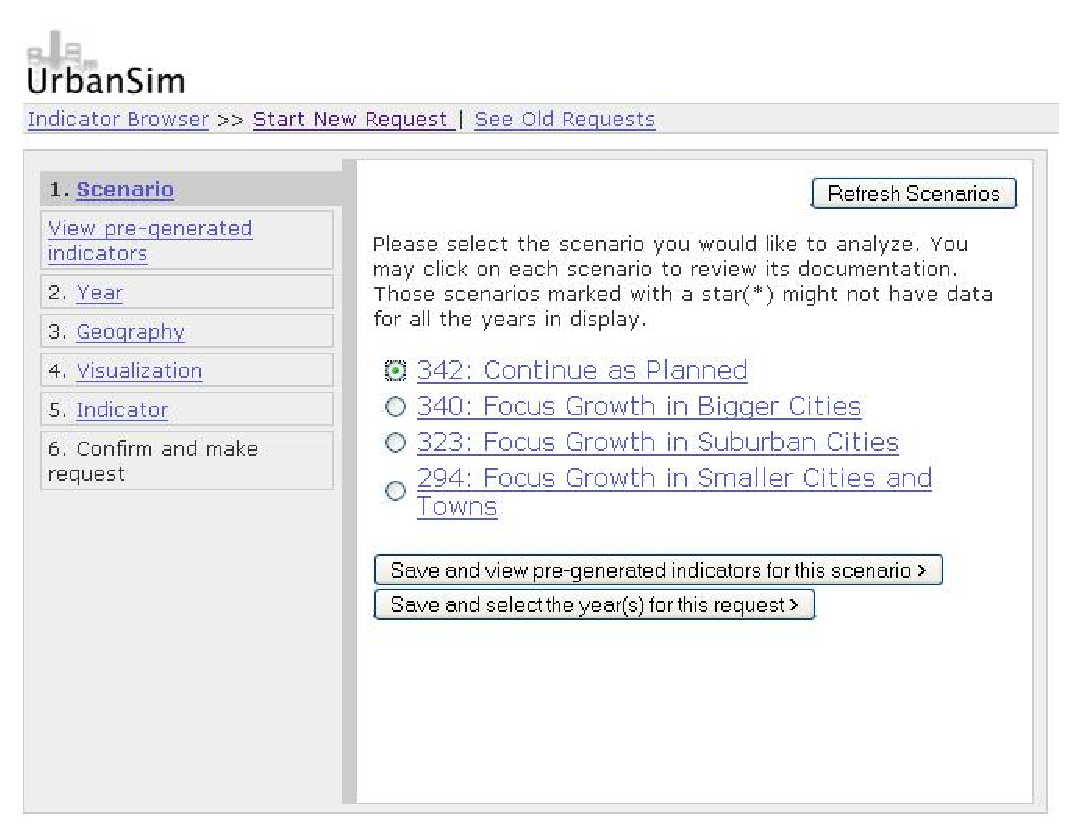
\includegraphics[width=3in]{figs/scenario_full}
\caption{\label{fig:scenario_full} Indicator Browser screenshot. The 
Session Bar on the left keeps track of users' selections and
provides easy navigation throughout the interface.}
\end{figure}

The Indicator Browser is a web-based tool for browsing through different
UrbanSim runs, and indicator values that have already been computed for those
runs and their visualizations.  It also allows new indicator values and
visualizations to be requested, using a web-based form. It is
intended to make indicators easier to generate by the interface's target users. 
It is also intended as a 
step towards including more of the indirect stakeholders into
the direct stakeholder group.  Its design and implementation is strongly
informed by the Value Sensitive Design work, in particular, the empirical
results on the usefulness of providing tools that contain ready-to-hand information, and on
transparency.

In addition, the design and testing of the Indicator Browser made extensive
use of user-centered design techniques, including iterative design, paper
prototyping, and frequent design discussions and user feedback.  
The intended users
are urban modelers and planners, as well as software developers.  Each
iteration was designed and evaluated using interactive or paper prototypes
keeping in mind the values that UrbanSim is meant to explicitly support.  A
brief description of all these methodologies, as well as their specific
application for the Indicator Browser, follow below.

\subsection{Iterative User Interface Design}

Iterative user interface design is by now standard practice in the Human Computer
Interaction (HCI)
community (see e.g.\ \cite{nielsen-ieee-computer-1993}).  It is based on
the realization that even the best designers will not design the ideal
interface on the first attempt; instead, iterative testing, feedback, and
refinement is essential in order to determine where and how to allocate
design efforts.  There is a continuing cycle of design, testing, and
feedback to the design.

%results page and session bar
\begin{figure}
\centering
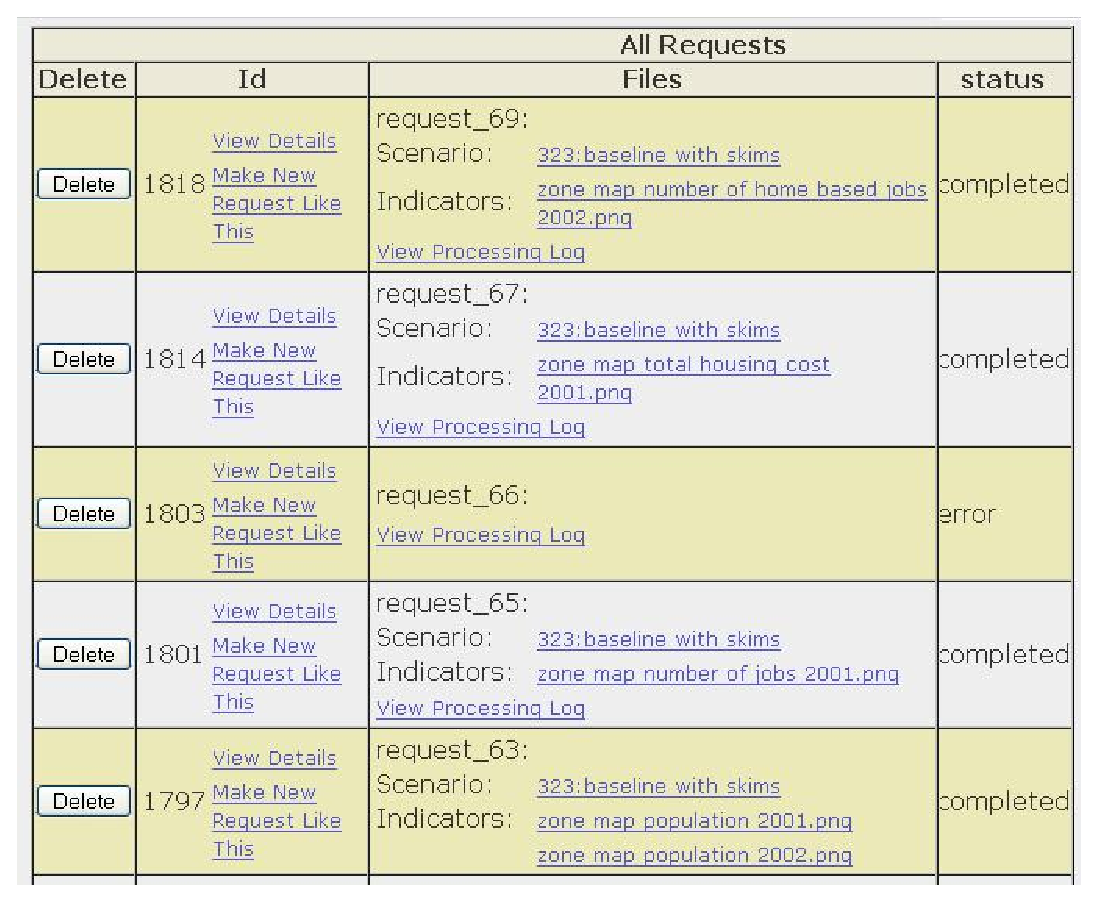
\includegraphics[width =3in]{figs/results}

\caption{\label{fig:results} Results Page, which contains
information about current as well as previous requests, and provides
commands to view details, delete requests, and make requests like
previous ones.}
\end{figure}

\subsection{Paper prototyping}

%scenario indicator and years page
\begin{figure*}
\centering
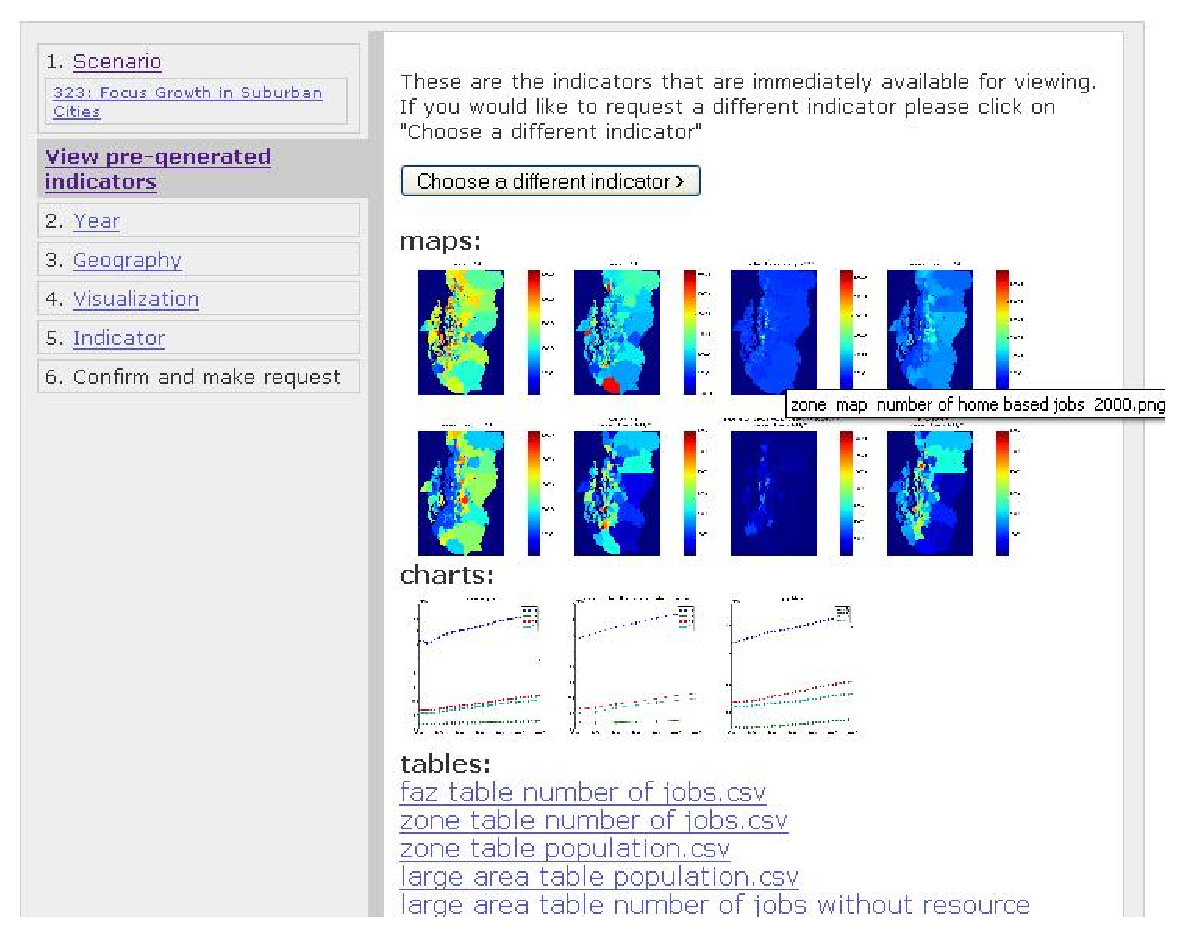
\includegraphics[width=7in]{figs/pregenerated}

\caption{\label{fig:pregenerated} Pre-generated
Indicators page, which displays all the indicators that are immediately
available for viewing.}
\end{figure*}

Paper prototyping originated in the Participatory Design work in
Scandinavia in the 1970s and 80s \cite{greenbaum-pd-1991}, but has since
become widely used as part of iterative user interface design techniques
\cite{rettig-cacm-1994}.  It is used to evaluate interfaces in the early
stages of the design process, with the goal of fixing as many usability
problems as possible before implementing the system. Although there are
certain interface affordances that paper prototypes simply cannot capture
(such as the experience of clicking a button), addressing design decisions
such as selecting feature sets and basic user-interface interactions using
paper prototypes lowers the design and implementation costs while having
tremendous impacts on the usability of the interface
\cite{nielsen-alertbox-paper-prototyping}.

The Indicator Browser design process combined usability testing,
iterative user-interface design via paper prototyping, and the Value
Sensitive Design methodology.  The principal goal in the Indicator Browser
design work has been for it to be usable by the target users
while continuing to support UrbanSim's core values.

\subsection{The Design Process} 

The Indicator Browser was designed through iterative user-interface design.
There was an informal initial discussion with modelers and planners at the
PSRC, which resulted in an initial sketch of the interface.  This interface
would be a single web page that would let users select the scenario that
they wished to visualize, along with specifications about the
visualization, such as its type, years, geography and of course, the
indicator(s) selection. After some technical investigations, the designers
found the implementation of this interface challenging due to the
dependencies between these selections, which are discussed 
in the next section. Therefore, the
designers moved to a sequential interface, in which the user's choices on
one web page would affect the content and available options for subsequent
pages.  The first author then performed a small informal interface
evaluation and fixed some usability issues to get the interface ready for
user interface evaluations.

Finally, two rounds of interface evaluations using rapid paper prototyping
were performed with eight urban modelers and planners at UrbanSim and
PSRC in May and June of 2005, respectively. A team of researchers
designed paper prototypes by printing the already existing Indicator
Browser web pages, sketching new pages using pencil and paper, and using
common stationary such as double-sided tape or stickers to create paper
widgets, for instance, drop-down menus or radio button selections.  The
interface design was refined by using the paper prototype to attempt to
complete a set of representative tasks. The tasks were developed using
personas that represented our target users, using the knowledge that some
of the researchers in the design team had about urban planning and our
target users.

The design team proceeded to evaluate the interface with volunteer
evaluators at PSRC and UrbanSim. As is usual with paper prototypes, one
person in the design team acted as a computer by reacting to user input
while the rest of the team recorded the user's experience. We asked our
users to think aloud, to say whatever was on their mind when they were
using the interface, in order to determine the interface's usability. We
were especially interested in determining which parts of the interface
worked well, so that we wouldn't alter them during the next round of
design, and which parts of the interface were confusing, in order to come
up with better design alternatives. In addition, we got suggestions
regarding the representative tasks, which we refined as well through the
multiple evaluations.  After the user completed the representative tasks we
asked them if they had any general suggestions and we explored possible
design alternatives together.
  
%\input{firsteval}

%\input{secondeval}

% LocalWords:  borning UrbanSim VSD UrbanSim's design's Habermas affordances UI
% LocalWords:  PSRC personas HCI yaels screenshot Pre

% $Id: recdesignissues.tex,v 1.11 2006/09/08 23:57:16 borning Exp $

\subsection{Recurring Design Issues}

There were some prevalent design issues throughout the interface
evaluation. These issues were discussed extensively and multiple design
alternatives were created in order to address them.

{\bf Providing ready-to-hand information.} This was a key goal,
both to support the value of transparency and also 
to enhance usability.  Its importance
is supported by our earlier empirical work (Section \ref{sec:prevwork}).  In
this context, the Indicator Browser should make all the information easily
available for the user to make an informed selection of the indicator to be
visualized.  In a larger context, interfaces often suffer from lack
of help and documentation in the right place \cite{nielsen-book-1994}.

Through the different stages in the design process, we found the need to
present the user with ready-to-hand information about UrbanSim, the
Indicator Browser, indicators and scenarios. The user wanted to know which
indicators had been precomputed, how long did the indicators take to
compute, the status of their request, what other requests had been
requested and the current visualization's selections. Since it was somewhat
difficult to assess how long were the indicators going to take due to the
complicated interaction amongst models during the simulation, we decided to
give the users a worst case estimate.
While some users were satisfied with this information, some still believed
more precision was necessary.

% *** is this right??? (which was that of three years). 

An example of our efforts to provide ready-to-hand information can be seen
in the results page found in Figure \ref{fig:results}, where the users can
see the status, details, results, computation and error logs for all the
requests.  We also provided links to the scenario run configuration details
and the indicator's Technical Documentation or code (in case the
documentation was not available). All of this information was highly
appreciated by the users at every step of the design process.

{\bf Sequence.} As previously noted,
the Indicator Browser was originally planned as a single-page
interface. However, this was not possible due to the
dependencies between selections. The indicator availability is dependent on
the geography one wants to visualize, since there are some indicators that
make more sense when visualized at certain aggregation levels. For
example, there are special Traffic Analysis Zones to study
transportation-related indicators.  Additionally, the visualization type
depends on which geography is selected, since not all visualizations are
possible for all geographies.  (For example, it is not practical to create
a table for gridcell-level indicators for most applications, since the
table would be too large.  The PSRC application, for instance, has
approximately 800,000 gridcells.)

The order of the choices presented to the user was designed based on a
combination of technical and empirical investigations.  For example, the
tests with paper prototypes indicated that users would prefer to select the
indicator before selecting details about the years, visualization type, and
aggregation levels (geography).  However, once we moved to the
implementation phase, we realized that constructing an Indicator required
knowledge about the selected years and geography, so in the implementation
the Indicator selection page was placed after these two selections.

{\bf Versatility vs.\ simplicity of design.}      
The Python script, which is the current way of generating indicators, is
very flexible and allows the user to create various indicators in addition to
the ones that are available through the existing
Opus attributes. In addition, users
who feel comfortable manipulating code can access UrbanSim's code directly
in order to manipulate the look and feel of the indicator
visualizations. Therefore, the design team had to come up with a design
that allowed for the most flexibility while maintaining its
usability. Consequently, there were several design tradeoffs that limited
the functionality of the interface in order to maximize its usability. One
example being that we only allow users to compare alternative scenarios to
the baseline scenario, rather than allowing them to compare any two
available scenarios.

{\bf Repetition reduction.} The interface is designed as a 
sequence of pages that present users with different 
alternatives in the form of radio buttons or check-boxes, in addition to
giving the users the option to provide a title for the request and an
email where to send the results. This meant that for every request they
had to go through the same set of pages, even if they only wanted to change
one or two alternatives. This proved to be very repetitive and
inefficient, especially since urban planners and modelers usually analyze
indicators starting with general information and then requesting more
specialized information where they see fit. For example, they might
initially want to see population maps at a county level and later request
the actual numbers (or a table) at a district level for a particular year
that looked interesting. Therefore, we decided to create a
feature called \emph{Make request like this}, which, when clicked, opens a new
window with a pre-filled request that the users can modify. This feature
was highly valued by the interface evaluators.

There were other shortcuts provided to reduce the amount of input
repetition, such as an \emph{All years} option in the years page that
automatically checked all the available years, a \emph{Results} page that
allowed users to browse through other users requests and retrieve their
visualizations. Finally, we also created a \emph{Pre-generated Indicators} page
for the users to have immediate access to a list of pre-generated
indicators after the scenario selection.

% LocalWords:  borning VSD UrbanSim gridcell gridcells UrbanSim's pre PSRC
% LocalWords:  tradeoffs

\section{System Overview}
This section provides a system perspective of AZ-SMART.  The system is a distributed configuration as depicted in Figure \ref{figSystem},
in which there are possibly different servers for the Geodatabase (ArcSDE and MS SQL Server), the land use model (OPUS), the travel model,
and potentially a web server (using ArcIMS or its successor).  Initially we expect that OPUS and ArcGIS will be running strictly on the
same machine.

The interface between ArcGIS and OPUS will be integrated through the ArcGIS user interface (described in more detail in the subsection on
user interface).  There may be situations in which a user wishes to run an OPUS client independently of ArcGIS, for example when focusing
on model estimation, or at times when controlling simulation runs, or in the use of a fully automated batch simulation linking the land
use and travel model systems.  Similarly, a user might want to have multiple OPUS Clients on different machines, but share an OPUS Server
on another machine, to take advantage of a fast server, for example.  The interface between OPUS clients and servers would use networking
infrastructure, though there may be no need for this infrastructure during the first phase of this project.

In the first phase, the OPUS client and server will be on the same machine as an ArcGIS workstation, with multiple installations, one
per user (or machine).  Data will be shared via the Geodatabase, and if desired also through a drive that is mapped from each of the
clients to share the cache directory containing simulation results.

\begin{figure}[h]
\begin{center}
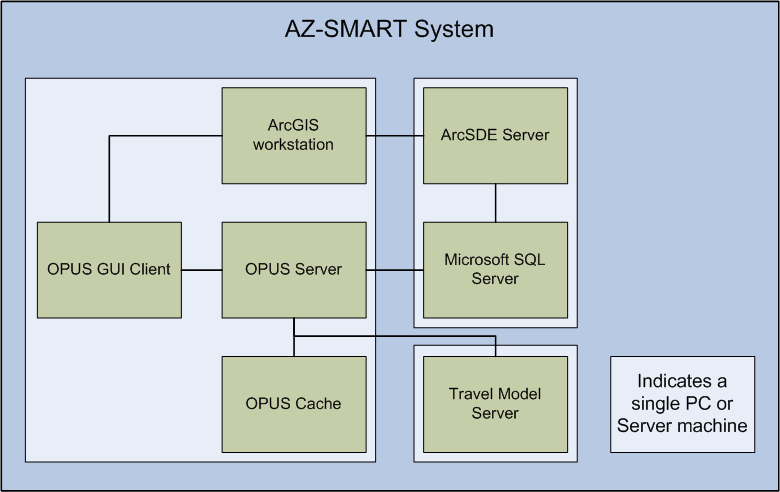
\includegraphics[scale=0.6]{figures/AZ-SMART_system_diagram.png}
\caption{AZ-SMART System Architecture}
\label{figSystem}
\end{center}
\end{figure}

%\newpage

% $Id: implementation.tex,v 1.7 2006/09/08 23:57:16 borning Exp $

\subsection{System Implementation}
\label{sec:implementation}

\subsubsection{Agile Test-first Software Development}

The Indicator Browser was developed using Agile Test-first software
development \cite{cockburn-book-2002}, which is a technique that focuses on
producing software systems in small steps driven by unit tests. The
idea is to deliver working software early and continuously to enhance
customer satisfaction. A developer should first write a test for a new piece
of functionality before it is implemented (test-driven development).  
Both independent modules and interactions between modules
are tested.  UrbanSim developers are encouraged to commit their code as
often as practical.  Fireman, a program that runs all the project's tests
every time the code is committed
to the source code repository, also aids in maintaining code quality.
Agile development encourages constant communication amongst the people
involved in the development process.  Developers write ``Today
messages'' \cite{brush-hicss-2005} every day to let the rest of the
development team know about their daily progress. In addition, software
engineers and project leaders meet with customers on a frequent basis to
communicate about the project's progress and redefine requirements.

\subsubsection{System Reliability and Robustness}

Robustness refers to the ability of the software system to perform
correctly even under extreme circumstances or when there are external or
internal changes that affect system's performance. Reliability refers to
the ability of the software system to perform as intended for a long
period of time.  Opus is an evolving system that constantly redefines its
requirements and whose code base is unstable.  However, the Indicator
Browser needs to be robust, reliable and flexible with respect to the
changes in the Opus code. Therefore, there were certain measures taken in
order to improve such reliability and robustness.

In order for the Indicator Browser to be reliable, all displayed indicators
should be able to be generated and visualized. To achieve this goal, we
created a set of Python unit tests that generate all possible indicator
visualizations under all possible visualization types for a small test
scenario run. The only indicators that are displayed on the interface are
those that passed the aforementioned test, therefore considerably improving
the chances that all the indicators displayed on the Indicator Browser can
in fact be successfully generated and visualized. Currently, these tests
and the set of available indicators are run and updated manually.  However,
these tests will be eventually added to the Opus nightly build and the
available indicator list will be updated automatically.

% LocalWords:  borning UrbanSim

% $Id: evaluation.tex,v 1.12 2006/09/08 23:57:16 borning Exp $

\section{Evaluation}
\label{sec:evaluation}

The Indicator Browser was evaluated by four urban planners and two UrbanSim
developers in April 2006. The evaluation consisted of an observation of the
use of the Indicator Browser in a natural setting, followed by an informal
interview guided by five general questions.  The users were asked to
generate and visualize the indicators that they usually work with using our
interface. If they were unclear about what indicators to generate, the
evaluator prompted them to generate the indicators that were discussed on
one of the PSRC-UrbanSim meetings that was held a few days before the
evaluation.  The users were asked how often and how they usually generate
and visualize indicator visualizations. They were asked to compare the
Indicator Browser with the tools they currently use. They were also asked
whether and how they would use the Indicator Browser, and what changes
needed to be made for the interface to be useful for them. Finally,
they were asked to consider whether this interface could be used by a
different set of users and if so, who would that group be. We were
interested in gauging how commonplace it was for the users to generate or
visualize indicators.  Since there are two different types of users: urban
modelers and planners on the one hand, and UrbanSim developers on the other,
each group might have a
different set of needs and uses for the Indicator Browser. Furthermore, we
wanted to prioritize the usability issues found during the evaluation and
to have an understanding of possible future steps.

\subsection{Usability and Value Issues}

% *** COULD SHORTEN OR EVEN SKIP THIS SECTION ***

The evaluations showed that there are still some usability issues to fix
before deploying the interface.  Some of the interface changes made after
the second round of usability testing, mainly due to internal design
discussions, had not been evaluated before and showed the need for
refinement. For example, we added a feature that allowed users to see
pre-generated indicators immediately after the scenario selection (Figure
\ref{fig:pregenerated}).  If the indicator that the user wanted wasn't on
the list there was a \emph{Choose a different indicator} button that allowed
them to continue making their request. This was a very useful feature that
the users liked.  The users showed interest once again in having 
more ready-to-hand information, such as having the scenario's name 
for each of the requests on the results page.

\subsection{Post-task Interview}

After the users interacted with the interface for about half an hour the
evaluator asked them the following five questions:

\begin{itemize}
\item How often and how do you currently generate indicator visualizations?
\item How does the Indicator Browser compare to the tools you currently use
  to generate indicator visualizations?
\item Would you use the Indicator Browser? If so, how?
\item What would need to be fixed for you to use the Indicator Browser?
\item Would you recommend this interface to someone else? If so, who?
\end{itemize}

The interviews revealed that each of the user groups generate indicators
with different frequency and that they have different perspectives on how
useful currently used tools are based on generation frequency and level of
programming expertise.  Their perception of the utility of the currently
used tools had an impact in their perception of utility of the Indicator
Browser.

One of the users is a general urban planner who usually does not generate
indicators himself. The indicators are generated for him and he can access
them through a file server.  He then visualizes them using the
FastStone Image Viewer tool (\url{http://www.faststone.org}), which allows
contiguous visualization of up to four images, as well as synchronized
image zooming and panning. Consequently, he did not find the indicator
generation mechanism extremely helpful for his common work tasks. He
mentioned he usually looks at the same set of indicators, and so he would
use this interface to see the pre-generated indicators and would most
likely not create some of his own.  However, he suggested that the
interface would be a useful way for the general public to access this
information.

Two of our interface evaluators are urban modelers and generate indicators
on a regular basis. Although they know how to create macros and how to
program, they felt much more comfortable generating indicators through a
web application. They found the Python script (described in Section
\ref{sec:opus}) to have a high set-up cost. The Python script requires them
to check out the correct projects from the source code
repository, set environment
variables, modify the Python script, and run it using multiple
applications.  Since several sub-processes are launched within the script,
the users became confused whenever windows popped on their screen which
they didn't know if they could close or what they were meant to do. 
This last user group found the Indicator
Browser very useful for indicator generation due to its low set-up cost,
aggregation of functions into a single web-based application, and the
elimination of the need to program. Their primary concern was with the
pre-generated indicators section of the interface, which they found
confusing, and mentioned they would
use the interface after this issue was resolved.

Two of our evaluators are software engineers and developers with the
UrbanSim project. They are very comfortable using and modifying the Python
script and enjoy the flexibility that it affords. The Python script allows
them to force color ramps on maps and create indicator difference,
aggregations and dis-aggregations of data across multiple levels of
geography. However, they do not have direct access to the file server at
home. One of the evaluators mentioned he had to use Microsoft's Remote
Desktop application to access the generated indicators from the UrbanSim
file servers. Therefore, he found the Indicator Browser to be useful for
accessing the indicators using a web browser from any
location. The second evaluator liked the organization of information. He
liked that he could see which scenarios were available and that he could
access the indicators by selecting the scenario from a list on a webpage
rather than having to find out what the scenario directory was through
database tables and access it through the file server.  He mentioned that
once he analyzes the outcome of the big batch of indicators generated
through the script he would use the Indicator Browser to create additional
indicators instead of editing and rerunning the script. However, the
other software engineer mentioned that he would not use the Indicator
Browser since he enjoys the Python script functionality and does not like
using multiple applications to complete a single task.

Some users mentioned they would recommend this interface to the general
public and activist groups for use in urban planning courses, engaged
citizens workshops, technical advisory committees and general regional
policy inquiries.

All users found emailing the results or accessing the results through a URL
to be very useful. Most of them mentioned they would use the Indicator
Browser to create additional indicators to get more detailed information
after analyzing the pre-generated indicators.


% LocalWords:  borning UrbanSim PSRC  pre FastStone EMPAL FAZ Fortran gauging
% LocalWords:  webpage

% $Id: conclusion.tex,v 1.6 2006/06/02 19:02:35 borning Exp $

\section{Conclusion and Future Work}

In this chapter we have presented an introduction to the domain of urban
modeling and to some of the uses and controversies around employing these
models to inform public decision-making, including a taxonomy of refinements
to urban models and to the process of applying them.  We then presented a
case study of the UrbanSim model system, including principal areas of
research and some applications to planning activities in different regions.
This domain represents a significant opportunity for digital government
research: hard technical problems, unmet demand from government users, and
important issues around supporting a more democratic planning process.

There is work that remains to be done.  Most importantly, our goal
of producing a system that is in routine and widespread use in
informing the planning process is not yet achieved.  UrbanSim is
being transitioned to operational use in a number of regions, and
there are a fair number of additional research applications of the
system.  However, it is not yet in routine policy use.  Beyond that,
the development of the Opus platform should enable a rich set of
collaborations among researchers world-wide, including the
development of open-source travel models and environmental models
closely integrated with the land use models in UrbanSim.  Finally,
we have touched on two other major open areas of ongoing research:
first, increasing access to the results of modeling for a wide range
of stakeholders, and ultimately to simulating additional
alternatives; and second, providing a principled modeling of
uncertainty in land use and transportation simulations.

% LocalWords:  borning pwaddell UrbanSim

% $Id: ack.tex,v 1.7 2006/09/05 00:48:10 borning Exp $

\section*{Acknowledgments}

We would like to thank all of the UrbanSim research team members and
collaborators, in particular Janet Davis and Sandra Fan for help with the
initial rounds of design and evaluation of the system described here; Batya
Friedman, Janet Davis, and Peyina Lin on their work on the design of the
Indicator Browser and interaction mechanism, on which this work draws
heavily; David Socha for software engineering help; Bjorn Freeman-Benson,
Casey Huggins, and Jonathan Fuchs for their work on the previous versions
of the system; and the participants in all of our user studies.  This
research has been funded in part by grants from the National Science
Foundation (EIA-0121326 and IIS-0534094).

% LocalWords:  borning UrbanSim Batya Peyina Socha EIA IIS yaels



% conference papers do not normally have an appendix

% use section* for acknowledgement
% optional entry into table of contents (if used)
% \addcontentsline{toc}{section}{Acknowledgment}

% trigger a \newpage just before the given reference
% number - used to balance the columns on the last page
% adjust value as needed - may need to be readjusted if
% the document is modified later
%\IEEEtriggeratref{8}
% The "triggered" command can be changed if desired:
%\IEEEtriggercmd{\enlargethispage{-5in}}

% references section
% NOTE: BibTeX documentation can be easily obtained at:
% http://www.ctan.org/tex-archive/biblio/bibtex/contrib/doc/

% can use a bibliography generated by BibTeX as a .bbl file
% standard IEEE bibliography style from:
% http://www.ctan.org/tex-archive/macros/latex/contrib/supported/IEEEtran/bibtex
%\bibliographystyle{IEEEtran.bst}
% argument is your BibTeX string definitions and bibliography database(s)
%\bibliography{IEEEabrv,../bib/paper}
%
% <OR> manually copy in the resultant .bbl file
% set second argument of \begin to the number of references
% (used to reserve space for the reference number labels box)
% \begin{thebibliography}{16}
% \input{bibliography}
% \end{thebibliography}

\bibliographystyle{IEEEtran}
\bibliography{../bibliographies/urbansim}

\end{document}

% LocalWords:  borning UrbanSim Yael Schwartzman BBND yaels
